\documentclass[11pt, letterpaper, includehead]{article}

%%%%%%%%%%%%%%%%%%%%% Pre-document %%%%%%%%%%%%%%%%%%%%%
\usepackage{fancyhdr}  % Allow for headers
\usepackage{graphicx}  % Allow for figures 
\usepackage{float}     % Allow for figure inserted in specified location
\usepackage{array}     % Allow for cell width manipulation
\usepackage{nicematrix}
\usepackage{multicol} % Multiple cols
\usepackage{tikz} % For latex graphics

\setlength{\parindent}{0pt} % Remove auto paragraph indents

% Get rid of those big ass margins
\usepackage[margin=1in]{geometry}

% Table cell formatting
\setlength{\arrayrulewidth}{0.25mm}
\setlength{\tabcolsep}{11pt}
\renewcommand{\arraystretch}{1.2}

\begin{document}

%%%%%%%%%%%%%%%%%%%%% Title Page %%%%%%%%%%%%%%%%%%%%%
\begin{titlepage}
  \begin{center}
    \Huge{\textbf{Lab 6}}\\
    \Huge{When Pigs Fly}
    \vfill
    \begin{figure}[H] % H makes the figure insert at the position in the document
      \centering
      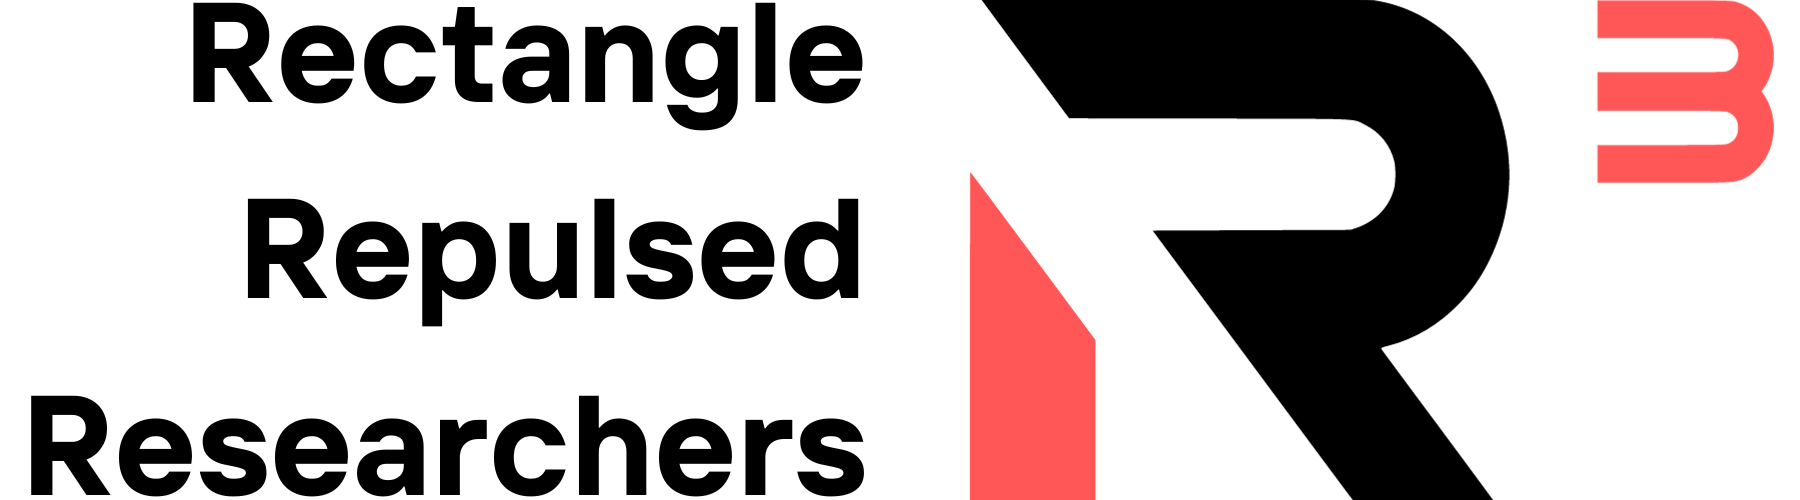
\includegraphics[width=6cm]{../logo.png}
    \end{figure}
    \large{\textbf{your name here}}\\
    \large{Julian Barossi, Liam Gilligan, Stephanie L'Heureux}\\
    \vspace{0.5cm}
    \normalsize
    \today
  \end{center}
\end{titlepage}

%%%%%%%%%%%%%%%%%%%%% TABLE OF CONTENTS %%%%%%%%%%%%%%%%%%%%%
\tableofcontents
\pagebreak % Move to next page

% Add a nice fancy header
\pagestyle{fancy}
\fancyhead{}
\fancyhead[C]{\textbf{Lab 5:} Forces and Acceleration}

%%%%%%%%%%%%%%%%%%%%%%%% SECTION 1 %%%%%%%%%%%%%%%%%%%%%%%%

\section{Set Up and Data Taking}


\renewcommand{\arraystretch}{2} 
\subsection{Measured values}
\begin{center}
  \begin{tabular}{|  m{5cm} | m{4cm} | m{3cm} | }
    \hline
    \textbf{Quantity} & \textbf{Value} & \textbf{SI units} \\
    \hline
    Mass  (m)  & $110.5g\left( \frac{1kg}{10^3g}\right)$ & $0.1105 kg$  \\
    \hline
    Diameter of cylinder ($\Delta x$) & $1in\left( \frac{0.0254m}{1in}\right)$ & $0.0254 m$  \\
    \hline
    Radius (r) & $48.25 cm \left( \frac{1m}{10^2cm}\right)$ & $0.4825 m$  \\
    \hline
  \end{tabular}
\end{center}
\renewcommand{\arraystretch}{1.5}

\section{Analyzing the Data}
\subsection{Absolute value of the force}
The tension $T$ was found to be $1.28136N$ using the force sensor.

\subsection{Centripetal force from measured tension}
\begin{center}
  \begin{tikzpicture}
    \draw[thin,dashed][->] (-2,0) -- (2,0) node[right] {$x$}; % x axis
    \draw[thin,dashed][<-] (0,-2) -- (0,2) node[above] {$y$}; % y axis
    \draw[very thick, blue][->]  (0,0) --  node [right, pos=1, color=black] {$T$} (0,1.5); % tension
    \draw[very thick, blue][->]  (0,0) -- node [right, pos=1, color=black] {$mg$} (0,-1); % weight
    \draw[fill=black] (0,0) circle (0.08); % point in the center
  \end{tikzpicture}
\end{center}
$$\sum F_r = T - mg$$
$$\sum F_r = (1.28136N) - (0.1105 kg)(9.8 m/s^2)$$
$$\sum F_r = 0.19846N \approx 0.198N$$
$$\boxed{\sum F_r = 0.198N}$$

\subsection{Speed at the lowest point}
\begin{center} 
  \begin{tabular}{|  m{1.5cm} | m{3.2cm} | m{3.2cm} | m{3.2cm} | } 
    \hline
    \textbf{Attempt} & \textbf{Tension (N)} & \textbf{Time (s)} & \textbf{Speed (m/s)} \\ 
    \hline
    1 & 1.28136 & 0.0265139 & 0.9579880742 \\ 
    \hline
  \end{tabular} 
\end{center}

$$v = \frac{\Delta x}{t}$$
$$v = \frac{0.0254 m}{0.0265139s}$$
$$v = 0.9579880742...m/s \approx 0.958 m/s$$
$$\boxed{v = 0.958 m/s}$$

\subsection{Centripetal force from measured times}
\subsubsection{Calculations}
$$\sum F_r = ma_r$$
$$\sum F_r = (m)\left( \frac{v^2}{r}\right)$$
$$\sum F_r = (0.1105 kg)\left( \frac{(0.9579880742m/s)^2}{0.4825 m}\right)$$
$$\sum F_r = 0.21018...\approx 0.210N$$
$$\boxed{\sum F_r = 0.210N}$$

\subsubsection{Percent difference}
Let the force found using the tension be A and the force found using the time be B.
$$\%diff = \frac{|A - B|}{(A + B)/2}$$
$$\%diff = \frac{|0.198N - 0.210N|}{(0.198N + 0.210N)/2}$$
$$\%diff = 0.059$$

\subsection{Data from five recordings}
% The spread sheet is wrong lol

How do your measured values of centripetal force compare to the calculated
values?\\
What are possible reasons for the differences between the measured and
calculated values of centripetal force? \\

\section{When pigs fly}

\subsection{Free body diagram}
\begin{multicols}{2}
  \centering
  \begin{tikzpicture}
    \draw[thin,dashed][->] (-2,0) -- (2,0) node[right] {$x$}; % x axis
    \draw[thin,dashed][->] (0,-2) -- (0,2) node[above] {$y$}; % y axis
    \draw[very thick, blue][->]  (0,0) --  node [right, pos=1, color=black] {$T$} (1.5,1.5); % tension
    \draw[very thick, blue][->]  (0,0) -- node [right, pos=1, color=black] {$mg$} (0,-1.5); % weight
    \draw[fill=black] (0,0) circle (0.08); % point in the center
    \draw (0,0.5) node[right] {$\theta$}; % point in the center
    % \draw (0,0) ++(0:2) arc (0:45:2); % point in the center
    % \draw[blue] (0,0) arc[start angle=-45, end angle=90, radius=1];
  \end{tikzpicture}

  \columnbreak

  \begin{tikzpicture}
    \draw[thin,dashed][->] (-2,0) -- (2,0) node[right] {$x$}; % x axis
    \draw[thin,dashed][->] (0,-2) -- (0,2) node[above] {$y$}; % y axis
    \draw[very thick, blue][->]  (0,0) --  node [below, pos=1, color=black] {$T\sin(\theta)$} (1,0); % tension
    \draw[very thick, blue][->]  (0,0) --  node [right, pos=1, color=black] {$T\cos(\theta)$} (0,1); % tension
    \draw[very thick, blue][->]  (0,0) -- node [right, pos=1, color=black] {$mg$} (0,-1.5); % weight
    \draw[fill=black] (0,0) circle (0.08);
  \end{tikzpicture}
\end{multicols}

\subsection{Derive equation of theoretical speed}
\begin{multicols}{2}
  \center{\textbf{x-axis}}
  $$\sum F_x = ma_x$$
  $$\sum F_x = m\left(\frac{v^2}{r}\right)$$
  $$T\sin(\theta) = m\left(\frac{v^2}{r}\right)$$

  \columnbreak
  \center{\textbf{y-axis}}
  $$\sum F_y = ma_y$$
  $$\sum F_y = 0$$
  $$T\cos(\theta ) = 0$$
\end{multicols}

\subsection{Theoretical speed}

\subsection{Measured values}

\renewcommand{\arraystretch}{2} 
\begin{center}
  \begin{tabular}{|  m{5cm} | m{4cm} | m{3cm} | }
    \hline
    \textbf{Quantity} & \textbf{Value} & \textbf{SI units} \\
    \hline
    Radius (r)  & $60.5 cm\left( \frac{1m}{10^2cm}\right)$ & $0.605 m$  \\
    \hline
    Length of string (L)  & $97 cm\left(\frac{1m}{10^2cm}\right)$ & $0.97m$ \\
    \hline
  \end{tabular}
\end{center}
\renewcommand{\arraystretch}{1.5}
For the period (T), we minimized human error by measuring the time for five revolutions then found the period 
by dividing by five. To further limit inaccuracies, this was repeated five times. For the period value, we 
took the average of these measurements.
\begin{center} 
  \begin{tabular}{|  m{2cm} | m{5cm} | m{5cm} | } 
    \hline
    \textbf{Attempt} & \textbf{Five revolutions (s)} & \textbf{One revolution (s)}\\ 
    \hline
    1 & 8.63 & 1.726 \\ 
    \hline
    2 & 8.68 & 1.736 \\ 
    \hline
    3 & 8.62 & 1.724 \\ 
    \hline
    4 & 8.61 & 1.722 \\ 
    \hline
    5 & 8.59 & 1.718 \\ 
    \hline
    \hline
    \multicolumn{2}{|l|}{{\textbf{Average period}}(\boldmath{$\bar{T}$})} & 1.7252 \\ 
    \hline  
  \end{tabular} 
\end{center} 

\subsection{Experimental speed}
$$v = \frac{2\pi r}{T}$$
$$v = \frac{2\pi (0.605 m)}{1.7252s}$$
$$v = \frac{1.21 \pi m}{1.7252s}$$
$$v = 2.203412421...m/s \approx  2.203m/s$$
$$\boxed{v_{exp} = 2.203m/s}$$

\subsection{Percent difference}
$$\%diff = \frac{exp - thy}{thy} \times 100\%$$
$$\%diff = \frac{v_{exp} - v_{thy}}{v_{thy}} \times 100\%$$
$$\%diff = \frac{2.203m/s - v_{thy}}{v_{thy}} \times 100\%$$

\end{document}
